\chapter{Background} \label{ch:background}
\epigraph{From now on you shall be called Brian that is called Brian.}{The Life of Brian}
In this chapter, we introduce commonly used formalisms and definitions. We start we classic First Order Logic, then proceed by introducing Answer Set Programming and Constraint Programming. Then, to help the reader we demonstrate a connection between the formalisms. After we describe Inductive Logic Programming and Pattern Mining.

\section{First Order Logic}
\begin{figure}[t]
  \centering
  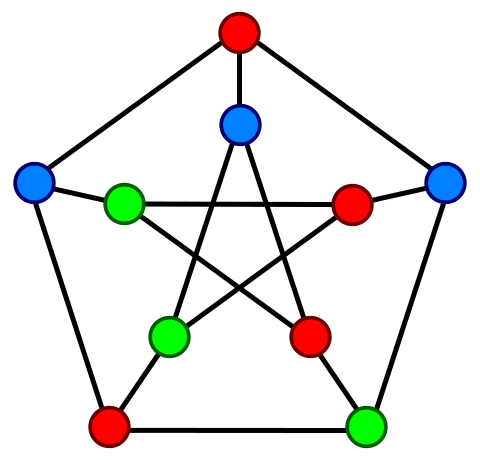
\includegraphics[width=0.4\textwidth]{Petersen_graph_coloring.png}
  \caption{Graph coloring of the Petersen's graph using three colors}
  \label{fig:petersen_coloring}
\end{figure}
In this section, we describe the syntax and semantics of \acrshort{fol},
for an extensive overview of \acrshort{fol}, we refer to \textcite{fo_overview}.

A formal language is a triple: \textit{vocabulary}, \textit{syntax} and \textit{semantics}. The vocabulary is the set of symbols that can be used. The syntax is the set of rules on how these symbols can be combined together. And the semantics is the way to interpret the statements. We omit the vocabulary, when it is clear from the context.

For each predicate $p$ and each function symbol $f$ in the vocabulary, we assume a natural number $n$ called \textit{arity} to be given, written as $p/n$ and $f/n$. This number indicates the number of parameters it takes; we often omit the arity when it is clear from the context. Propositional symbols are zero-arity predicates and constants are zero-arity functions. 
We assume propositional symbols \textit{true} and \textit{false}, whose domains are $\top$ and $\bot$ correspondingly, to be always in the vocabulary.

\begin{example}[Predicates and functions]\label{example:predicates_and_functions}
  Consider the famous problem of coloring a map, as in Figure \ref{fig:petersen_coloring}. The vocabulary would contain a predicate symbol \textit{border/2} and a function \textit{coloring/1}, together with a set of constants representing countries, such as \textit{belgium}, \textit{netherlands}, etc.
\end{example}

A \textit{structure} associates values with the predicates and functions from the vocabulary. A structure $I$ consists of

\begin{itemize}
  \item A domain $D^I$, which we also refer to as the \textit{universe}. The domain defines what are the possible values to be used.
  \item For each predicate $p/n$, the set of its values $p^I \subseteq \overbrace{D^I \times \dots \times D^I}^{n}$
  \item For each function symbol $f/n$,  $f^I$ the mapping  $\overbrace{D^I \times \dots \times D^I}^{n} \mapsto D^I$
\end{itemize}
We call the set of values $p^I$ for a predicate $p$  and the mapping $f^I$ for a function $f$ an \textit{interpretation}.

We assume the set of inequalities $\{ =, \neq, <, >, \leq, \geq \}$,  arithmetic $\{+, -, *, \div \}$ and true $\top$, false $\bot$ to be interpreted by any interpretation in a standard way.

\begin{example}[Interpretaion of map coloring]
  Consider the predicate and the function from Example \ref{example:predicates_and_functions}. Then, $I$ can be the following:
  \begin{itemize}
    \item Domain $D^I = \{ \textit{red, green, blue, belgium, netherlands, germany, france} \}$
    \item The interpretation $\textit{border}^I = \{ (\textit{belgium, netherlands}), \dots \}$                                                                                     
    \item The interpretation $\textit{coloring}^I = \{ \textit{belgium} \mapsto \textit{green}, \dots \}$                                                                                     
  \end{itemize}
\end{example}


\paragraph{Syntax} 

The syntax of \acrlong{fol}, such as valid terms and formulae, is defined inductively.

A \textit{term} is defined as follows  
\begin{itemize}
  \item a \textit{variable} is a term
  \item if $t_1,\dots,t_n$ are terms and $f/n$ is a function, then $f(t_1,\dots,t_n)$ is term
\end{itemize}
We say a term $t$ is a \textit{domain term}, if $t$ is in the domain.


A \textit{formula} is defined as follows

\begin{itemize}
  \item if $p/n$ is a predicate and $t_1,\dots,t_n$ are terms, then $p(t_1,\dots,t_n)$ is a formula, called an \textit{atom}  
  \item if $\phi$ is a formula, then $\lnot \phi$ is a formula
  \item if $\phi$ is a formula and $x$ is a variable, then $\forall x: \phi$ and $\exists x: \phi$ are formulae 
  \item if $\phi$ and $\psi$ are formulae, then $\phi \wedge \psi$ and $\phi \vee \psi$ are formulae
\end{itemize}

We call a \textit{literal} an atom or the negation of an atom. An expression of the form $a \rightarrow b$ is a shorthand for $\lnot a \vee b$, and $a \leftrightarrow b$ is a shorthand for $a \rightarrow b \wedge b \rightarrow a$. A \textit{sentence} is a formula without free, i.e., non-quantified, variables. A set of sentences  is called a \textit{theory}.

\begin{example}[Formula]\label{example:formula}
  As in previous examples, we consider the problem of map coloring. The following formula:
  \begin{equation*}
    \forall X,Y{:}~\textit{border}(X,Y) \rightarrow \textit{coloring}(X) \neq \textit{coloring}(Y)
  \end{equation*}
has an indented meaning of enforcing the colours of adjacent countries to be different.
\end{example}


\paragraph{Semantics}
The semantics is defined inductively over the structure of the terms and of the formulae.

Let $I$ be a structure and $t$ be a domain term, then the \textit{value} of $t$ is $t^I = d$, where $d$ is the domain element. If $t$ is an expression of the form $f(t_1,\dots,t_n)$, then its value is $f^I(t_1^I,\dots,t_n^I)=d$, where $d$ is the domain element.

The truth assignment of a structure $I$ over formulae is defined inductively as follows:

\begin{itemize}
  \item $p(t_1,\dots,t_n)^I$ is true, iff $p^I(t_1^I,\dots,t_n^I)$ is true
  \item $(\lnot \phi)^I$ is true, iff $\phi^I$ is false
  \item $(\phi \wedge \psi)^I$ are true, iff $\phi^I$ and $\psi^I$ are true
  \item $(\phi \vee \psi)^I$ are true, iff $\phi^I$ or $\psi^I$ are true
  \item $\forall X: \phi$ is true, iff for each $d$ in $D^I$, $\phi[X/d]^I$ is true\footnote{$\phi[X/d]$ is a formula $\phi$, where each occurrence of $X$ is substituted with $d$}
  \item $\exists X: \phi$ is true, iff there is $d$ in $D^I$ such that $\phi[X/d]^I$ is true
\end{itemize}

We say that $I$ is a \textit{model} of or $I$ \textit{satisfies} a sentence $\phi$ iff $\phi^I$ is true, written as $I \models \phi$.

\begin{example}[Formula evalution]
  Assume, that the domain contains only two countries \textit{belgium} and \textit{netherlands} and two colors \textit{green} and \textit{red}. Let us show that $I$ with $\textit{border}$ being true for $(\textit{belgium,netherlands})$ and \textit{coloring} mapping \textit{belgium} to \textit{green} and \textit{netherlands} to \textit{red} is a model of the formula in Example \ref{example:formula}.

  \begin{tabular}{l r}
$(\forall X,Y{:}~\textit{border}(X,Y) \rightarrow \textit{coloring}(X) \neq \textit{coloring}(Y))^I$  & iff \\
for all $d_1,d_2 \in D$ holds $(\textit{border}(d_1,d_2))^I \rightarrow (\textit{coloring}(d_1) \neq \textit{coloring}(d_2))^I$ & iff \\
for $d_1 \neq \textit{belgium}$ and $d_2 \neq \textit{netherlands}$  the formula holds trivially & and if\\
for $d_1  = \textit{belgium}$ and $d_2 = \textit{netherlands}$, then $(\textit{belgium}, \textit{netherlands})$ in $\textit{border}^I$ & and\\ 
$f(\textit{belgium})^I = \textit{green} \neq \textit{red} = f(\textit{netherlands})^I$ & holds since \\
$\textit{green} \neq \textit{red}$  is true &
  \end{tabular}
\end{example}


\paragraph{Herbrand Interpretation} The \textit{Herbrand Universe} is the set of all terms over the vocabulary without variables. A \textit{Herbrand Interpretaion} has the Herbrand Universe as its domain and interprets each symbol and function by itself. Any model that contains \acrlong{una} (\acrshort{una}) \parencite{UNA} and \acrlong{dca} (\acrshort{dca}) \parencite{DCA} are equivalent to a Herbrand model.


\section{Answer Set Programming}
\acrlong{asp} (\acrshort{asp}) is a logic programming paradigm for solving combinatorial and constraint optimization problems \parencite{whatisasp}.

Contrary to the programming language Prolog, which is based on a proof-theoretic approach to answer queries, ASP follows a model generation approach. It has been shown to be effective for a wide range of constraint satisfaction problems \parencite{ASPbook}.

The remainder of this section introduces the essentials of ASP in a rather informal way. ASP is a rich (and technical) research area, so we do not focus on technical issues as these would complicate the presentation, but rather refer the interested reader to \textcite{ASPbook,eiter,leone,whatisasp} for more details on this. For the actual implementation, we will use the clasp system \parencite{ASPbook,BrewkaCACM}.

\begin{definition}[Disjunctive datalog program]
  A disjunctive datalog program is a finite set of rules of the form: 
  \begin{equation*}
    a_1 \vee a_2 \vee \dots \vee a_n \leftarrow b_1, \dots, b_k, \textit{ not }c_1,\dots,\textit{ not }c_h 
  \end{equation*}
\end{definition}
where $a_1, \dots, a_n, b_1, \dots, b_k,c_1, \dots c_h$ are atoms of a function-free First Order language $L$. Each atom is an expression of the form $p(t_1,\ldots,t_n)$, where $p$ is a predicate name and $t_i$ is either a constant or a variable. We refer to the head of rule $r$ as $H(r) = \{a_1,\dots,a_n\}$ and to the body as $B(r) = B^{+}(r) \cup B^{-}(r)$, where $B^{+}(r) = \{ b_1, \dots, b_k \}$ is the positive part of the body and $B^{-}(r) = \{ c_1, \dots, c_h \}$ the negative. 

If a disjunctive datalog program $P$ has variables, then its semantics are considered to be the same as that of its grounded version, written as \textit{ground(P)}, i.e. all variables are substituted with constants from the Herbrand Universe $H_P$ (the constants occurring in the program). The semantics of a program with variables is defined by the semantics of the corresponding grounded version.

An interpretation $I$ w.r.t. to a program $P$ is a set of ground atoms of $P$. Let $P$ be a positive disjunctive datalog program (i.e. without negation), then an interpretation $I$ is called closed under $P$, if for every $r \in \textit{ground}(P)$ it holds that $H(r) \cap I \ne \emptyset$ whenever $B(r) \subseteq I$. 
\begin{definition}[Answer set of a positive program \parencite{eiter}]
An answer set of a positive program $P$ is a minimal (under set inclusion) interpretation among all interpretations that are closed under $P$.
\end{definition}

Let us introduce the concept of a reduct \parencite{whatisasp}.
\begin{definition}[Gelfond-Lifschitz reduct] 
A reduct of a ground program $P$ w.r.t. an interpretation $I$, written as $P^I$, is  a positive ground program $P^I$ obtained by: 
\begin{itemize}
   \item removing all rules $r \in P$ for which $B^{-}(r) \cap I \ne \emptyset$;
   \item removing the literals ``$\textit{not }a$'' from all remaining rules.
 \end{itemize}
\end{definition}
Intuitively, the reduct of a program is a program where all rules with bodies contradicting $I$ are removed and in all non-contradicting all negative ones are ignored. The interpretation $I$ is a guess as to what is true and what is false.

\begin{definition}[An answer set of a disjunctive program]
An answer set of a disjunctive program $P$ is an interpretation $I$ such that $I$ is an answer set of positive ground program $\textit{ground}(P)^I$. 
\end{definition}

\begin{example} Consider the following disjunctive Datalog program $P$.
  \begin{eqnarray*}
    a \vee c  \leftarrow  b. \quad \quad b  \leftarrow  a, \textit{ not }c. \quad \quad a.
  \end{eqnarray*}
If we take the interpretation $I=\{a,b\}$ of $P$ as candidate answer set, then the reduct $P^I$ 
is  
\begin{eqnarray*}
    a \vee c \leftarrow b. \quad \quad   b \leftarrow a. \quad \quad  a.
\end{eqnarray*}
and it is easily seen that $I$ is a minimal interpretation closed under $P^I$, and therefore an answer set. 
\end{example}

We also use a special form of disjunctive rules called \textit{choice rules} \parencite{ASPbook}:
\begin{equation*}
  v_1~\{ a_1, a_2, \dots a_n \}~v_2 \leftarrow b_1, \dots, b_k, \textit{ not }c_1,\dots,\textit{ not }c_h
\end{equation*}
where $v_1$ and $v_2$ are integer constants. The semantics are as follows: if the body is satisfied, then the number of true atoms in $\{ a_1, a_2 \dots a_n \}$ is from $v_1$ to $v_2$.

An aggregate atom is an atom that has the following form: $l \# \{ a_1, \dots ,a_n \} u$
where $l$ and $u$ are constant numbers, each $a_i$ is a literal. The atom is true in an answer set $A$ iff there are from $l$ to $u$ literals $a_i$ that are true in $A$.

Another construct is \textit{maximization} \parencite{ASPbook, leone} (\textit{minimization} is defined analogously) stated as $\#\textit{maximize}\{ a_1=k_1, \dots, a_n=k_n \}$, 
where $a_1, \dots, a_n$ are classic literals and $k_1, \dots, k_n$ are integer constants (possibly negative). The semantics of this constraint are as follows: a model $I$ is selected if the weighted sum of $[a_i]*k_i$ is maximal in $I$, where $[\cdot]$ are Iverson brackets, i.e. $[a]$ is equal to $1$ iff $a$ is true in $I$ and $0$ otherwise.

\begin{example}[Map Coloring in ASP]
  Let us demonstrate how the problem of map coloring discussed before can be expressed in ASP. 

  The first constraint ensures that the binary predicate \textit{coloring/2} is a function from nodes to colors and the second that if there are two nodes of the same color joined by an edge, then it is not a model.
\begin{lstlisting}[caption=ASP encoding of map coloring constraints, label=lst:example_asp_coloring,basicstyle=\ttfamily]
1 { coloring(X,C) : colors(C) } 1 :- node(X).

:- edge(X,Y), coloring(X,C1), coloring(Y,C2), C1 = C2.
\end{lstlisting}
\end{example}


\section{Constraint Programming}
A detailed introduction to \acrlong{cp}(\acrshort{cp}) can be found in the ''Handbook of Constraint Programming`` \parencite{handbookcp}. A basic concept here is of a variable $v$ which always has an associated domain $d$, a domain here is simply a set of constants. An example domain is the Boolean domain \{ True, False \}. A constraint $c$ is an expression of the form \textit{name(vars)}, where \textit{vars} is a list of variable names and \textit{name} is the type of constraints from a predefined set of constraint classes. Examples of classes of constraints are comparisons,   arithmetic operations, list and set constraints (all-different, permutations, etc). We denote a set of all variables as $V$, of all domains as $D$ and of constraints as $C$, then a triple $(V,D,C)$ is a constraint programming model and a \acrlong{csp} (\acrshort{csp}) is the problem of finding an assignment $A$ for $V$ over $D$ satisfying all constraints $C$.

Let us demonstrate how it is possible to model the map coloring problem in \acrshort{cp}\footnote{based on the encoding from www.hakank.org/minizinc/map.mzn}
\begin{lstlisting}
% number of countries
int: n; 
% [belgium,denmark,france,germany,netherlands,luxembourg]
array[1..n] of var 1..4: country; 
% the map (as a binary matrix)
array[1..n,1..n] of 0..1: connections; 

forall(i,j in 1..n where i < j /\ conn[i,j] = 1) (
              country[i] != country[j]
      )
\end{lstlisting}



\section{\fod and the IDP System}
The knowledge based language \fod is the extension of First Order Logic with a number of features, such as, inductive definitions and aggregates. The IDP system \parencite{idppaper} is the reasoning system that accepts as the input \fod language and is able to perform a number of reasoning tasks: such as finding logical models, model checking and theorem proving.

Let us illustrate an inductive definition and an IDP program by example, see Listing \ref{lst:idp_reachability}, where Reach(x,y) is an example of an inductive definition, defined via the base case and the inductive step (see the Theory part).
\begin{lstlisting}[caption=An example of an inductive definition in FO(.) and of an IDP program,label=lst:idp_reachability]
vocabulary V{
  type Node
  Edge(Node, Node)
  Reach(Node, Node)
}

theory T:V{
  { 
    Reach(x,y)<- Edge(x,y).
    Reach(x,y) <-?z : Edge(x,z) & Reach(z,y).
  }
}

structure S:V{
  Node = {1;2;3}
  Edge = {1,2; 2,3; 3,1} 
}
\end{lstlisting}

An IDP program has three parts: \textit{Vocabulary} that defines the terminology and concepts of a problem, \textit{Structure} that sets certain values to true or false, and \textit{Theory} introduces constraints.




\section{Comparison Between Terminologies}
Since some readers might be more familiar with Constraint Programming than with Answer Set Programming or First Order Logic, in Table \ref{tab:terminology_comparison} we present a terminologies comparison \parencite{phd_broes}.

In this thesis we use Answer Set Programming terminology, unless specified otherwise.
\begin{table}
  \centering
  \begin{tabular}{c | c | c}
    \textbf{First Order} & \textbf{Constraint Programming} & \textbf{Answer Set Programming}\\ \hline
    variable & --         & variable\\
    constant & Boolean variable   & constant \\
    sentence & constraint & rule/constraint \\
    predicate symbol & Boolean variable array & predicate symbol\\
    function symbol &  variable array & function symbol\\
    atomic sentence & -- & fact\\
    interpretation & assignment & set of atoms\\
    theory & model & program \\
    model & solution & answer set
  \end{tabular}
  \caption{Mapping between terms in ASP, CP and FO}
  \label{tab:terminology_comparison}
\end{table}


\section{Relational Pattern Mining}
The task of relational pattern mining is to mine queries in a logical and relational learning setting. Starting with the work the Warmr system \parencite{warmr}, there has been a line of work that focusses on the following frequent query mining problem \parencite{bagm,farmer,condensed_luc}:

\noindent
{\bf Given:} \vspace{-8pt}
\begin{itemize}
\item a relational database $D$,
\item the entity of interest determining the \keypred/1 predicate,
\item a frequency threshold $t$,
\item a language ${\cal L}$ of logical queries of the form $\keypred(X) \leftarrow b_1, ..., b_n$ defining $key/1$ ($b_i$'s are atoms).
\end{itemize}\vspace{-5pt}
{\bf Find:} all queries $c \in {\cal L}$ s.t. $\freqpred(c,D) \geq t$, where ${\freqpred(c,D) = |\{\theta \mid D \cup c \models key(X)\theta \}|}$.

Notice that the substitutions $\theta$ only substitute variables $X$ that occur in \keypred. 

Here we focus our attention on graph data, as this forms the simplest truly relational learning setting and allows us to focus on what is essential for extending the declarative modeling paradigm to a relational setting. 
 
As an example, consider a graph database $D$, represented by the facts 
\begin{equation*}
\{ \edge(g_1,1,2),~ \edge(g_1,2,3),~ \edge(g_1,1,3),~ \edge(g_2,1,2),~ \edge(g_2,2,3), \dots \},
\end{equation*}
where the ternary relation $\edge(g,e_1,e_2)$ states that in graph $g$ there is an edge between $e_1$ and $e_2$ (we assume graphs to be undirected, so there is also always an edge between $e_2$ and $e_1$). The frequency of $\textit{key}(K) \leftarrow \edge(K,B,C), \edge(K,C,D), \edge(K,B,D)$ in this database is 2 as the query returns $g_1$ and $g_2$. If $key(g)$ holds,  then the graph $g$ is subsumed by the query specified defined in the body of the clause for \keypred.
In this section we briefly recap the necessary background both from the field of pattern mining.

Let $\mi{D}$ be a dataset, $\patternspace$ a language for expressing pattern properties or defining subgroups of the
data, and $\mi{q}$ a selection predicate. %Then t
The task of pattern mining is to find $\mi{Th}(\patternspace,D, \mi{q})= \{\phi \in \patternspace\, |\, \mi{q}(D, \phi) \text{ is true}\}$ (see the seminal work by \cite{DBLP:journals/datamine/MannilaT97}). 

Pattern mining has been mainly studied for % in three settings: 
itemsets, sequences, graphs and queries. These settings are determined by the language of $\patternspace$. 


